% DRAFT prepared with Claude Code for Andrew Spiers, 18 October 2026.
% TODO before submission:
%  - add Thomas Osburn's affiliation (left blank below);
%  - verify every reference (entries compiled from the PRL draft and standard self-force citations);
%  - acknowledgments and funding.
\documentclass[aps,prd,twocolumn,superscriptaddress,nofootinbib,floatfix]{revtex4-2}
\usepackage{amsmath,amssymb}
\usepackage{graphicx}
\usepackage{bm}
\usepackage[colorlinks=true,linkcolor=blue!50!black,citecolor=blue!50!black,urlcolor=blue!50!black]{hyperref}
\usepackage{xcolor}
\graphicspath{{./}{../figures/prl/}{../figures/}{../PRL/}}

\renewcommand{\Re}{\operatorname{Re}}
\renewcommand{\Im}{\operatorname{Im}}
\newcommand{\dext}{\delta_{\rm ext}}
\newcommand{\PhiP}{\Phi^{\rm P}}
\newcommand{\PhiS}{\Phi^{\rm S}}
\newcommand{\PhiR}{\Phi^{\rm R}}
\newcommand{\Pres}{\Phi^{\rm res}}
\newcommand{\x}{\mathbf{x}}
\newcommand{\Lop}{\mathcal{L}_\ell}

\begin{document}

\title{Complex-contour regularisation of second-order point-particle sources:\\ a scalar toy model}

\author{Andrew Spiers}
\email{andrew.spiers@ucd.ie}
\affiliation{School of Mathematics and Statistics, University College Dublin, Belfield, Dublin 4, Ireland}

\author{Thomas Osburn}
\affiliation{~} % TODO: affiliation

\date{\today}

\begin{abstract}
Second-order self-force calculations require the solution of a field equation whose source diverges as the fourth inverse power of the distance from the small body.
That source is well defined only as a distribution, and its spherical-harmonic modes converge slowly near the particle.
Production calculations tame it with a puncture scheme, which needs a second-order puncture and an expensive angular integration of the singular--singular part of the source near the worldline.
Here we develop an alternative that is native to mode-by-mode calculations.
The radial coordinate of each mode equation is deformed onto a contour in the complex plane that passes around the particle.
On the contour, the source is regular, and the real part of the solution on the real axis reproduces the Hadamard finite part of the mode equation, including the delta-function content of the source, without a second-order puncture.
Nonlinear sources need care, because the imaginary part of a continued field, which we call its shadow, leaks into the real part of a product.
We avoid this by keeping every source on the contour linear in a single continued quantity: closed-form singular pieces are evaluated at complex radius by angular quadrature, while the integrable remainder built from the regular field is formed on the real axis, where it can be solved directly or continued onto the contour with a Cauchy integral.
We develop and test the method on a flat-space scalar model whose source reproduces the distributional structure of the gravitational case.
With an exact singular field the second-order field is recovered to seventeen digits.
With truncated punctures, the error equals the usual mode-truncation error of a real-axis puncture scheme; the contour adds no additional error and avoids the need for a second-order puncture.
We also show that, unlike real-axis finite-part integration, the contour does not amplify noise in numerically computed source samples.
\end{abstract}

\maketitle

{\hypersetup{linkcolor=black}\tableofcontents}

%=====================================================================
\section{Introduction}\label{sec:intro}

Since the first detection of gravitational waves from a binary black hole merger~\cite{LIGO2016}, gravitational-wave astronomy has grown into a mature observational science.
The planned space-based detectors LISA~\cite{LISA2017}, TianQin and Taiji will open the millihertz band, where extreme-mass-ratio inspirals (EMRIs) are a key target.
Modelling an EMRI waveform accurately enough to track its phase over the many thousands of orbital cycles in band requires the self-force approach to black hole perturbation theory~\cite{BarackPound2019,PoundWardell2021}, carried to second order in the mass ratio~\cite{Pound2012,Warburton2021,Wardell2023,Pound2020}.
Second-order self-force waveforms for quasicircular inspirals in Schwarzschild spacetime already agree remarkably well with numerical relativity~\cite{Wardell2023}, and the extension to spinning primaries and eccentric orbits is an active frontier. Additionally, studies have suggested that high-accuracy measurements of intermediate-mass-ratio inspirals~\cite{} may require third-order self-force contributions.

The second-order problem encounters problems not present in first-order calculations~\cite{}.
These problems arise because the source of the second-order field equation is the quadratic Einstein operator acting twice on the first-order metric perturbation.
Near the small body, the first-order perturbation behaves like the Coulomb field of a point mass, falling off as the inverse distance $\rho$, and the quadratic source therefore diverges like $\rho^{-4}$.
Such a source is not locally integrable: as a function it has no meaning on the worldline, and the field equation only makes sense once the source is defined as a distribution~\cite{MusaeusPoundUpton2026}.
A second, related difficulty is practical.
The source is built by coupling spherical-harmonic modes of the first-order field, and near the particle the coupled sum converges slowly, the so-called infinite mode-coupling problem~\cite{MillerWardellPound2016}.

Production calculations handle both difficulties with a puncture, or effective-source, scheme~\cite{BarackGolbourn2007,VegaDetweiler2008,WardellWarburton2015,PoundMiller2014,Upton2026}.
A puncture is a local analytic approximation to the singular part of the field, modelled on the Detweiler--Whiting singular field~\cite{DetweilerWhiting2003}.
Subtracting it from the full field leaves a residual that is smooth enough to be solved for numerically, with an effective source that is the original source minus the field equation applied to the puncture.
At second order this requires a second-order puncture, and the quadratic source itself is split according to which parts of the first-order field enter it: a singular--singular (SS) part built from the puncture alone, a singular--regular (SR) part built from the puncture and the first-order residual, and a regular--regular (RR) part built from the residual alone.
The SS part must be evaluated by two-dimensional angular quadrature at every radial grid point near the worldline, and in the Schwarzschild calculations of Upton \emph{et al.}~\cite{Upton2026} this single step dominates the cost of the whole computation, at about three million CPU hours.
Recently, Musaeus, Pound and Upton~\cite{MusaeusPoundUpton2026} showed that the second-order field equation can instead be written with a point-particle (``skeleton'') source, regularised by Hadamard's finite part together with a finite worldline term, with no second-order puncture at all.

In this paper we develop a third route, which is native to the ordinary differential equation mode-by-mode calculations used in practice\footnote{So-called m-mode calculations, which involve solving $r$-$\theta$ partial differential equations, are not considered in this work but are another viable approach to second-order self-force calculations~\cite{}. Considering a complex contour regularisation of the m-mode problem is potential future work.}.
Each spherical-harmonic mode of the field obeys an ordinary differential equation in the radial coordinate, with coefficients that are real and analytic away from the origin.
Nothing prevents us from integrating that equation along a path in the complex radial plane.
If the path leaves the real axis some finite distance before the particle and returns a finite distance after it, the point source is replaced by its natural analytic extension, an \emph{extended delta function} with a simple pole at the particle's radius, and the sources that diverge on the real axis become perfectly regular on the contour (Fig.~\ref{fig:intro}).
Back on the real axis, the real part of the solution is the physical field.
For a linear equation with a point source, this is an old idea, essentially the Sokhotski--Plemelj formulas of complex analysis~\cite{Muskhelishvili1953} in the guise of a numerical method.
Two new ingredients are needed to make it work at second order.
The first is a split of the first-order field into singular and regular parts that is consistent between the contour and three dimensions.
The second is a treatment of the quadratic source in which no product of two continued fields is ever formed, because such a product would mix the imaginary part of each field, which we call its \emph{shadow}, into the real, physical part of the solution.

\begin{figure}[t]
\centering
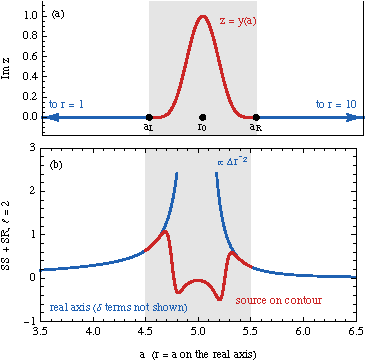
\includegraphics[width=\columnwidth]{prl_intro.pdf}
\caption{(a) The contour $z=y(a)$ in the complex $r$ plane (red). Outside the worldtube (shaded) the radial coordinate stays on the real axis (blue).
(b) The $\ell=2$ second-order source of the toy model, with an exact singular field. On the real axis (blue) the SS and SR sources together diverge as $\Delta r^{-2}$ at $r_0$; the $\delta$-function terms of SR are not shown. On the contour (red) the real part of the continued source is bounded and joins the real-axis source at the worldtube boundaries. Its imaginary part, the shadow, is shown in Fig.~\ref{fig:source}(b).}
\label{fig:intro}
\end{figure}

We develop and test the method on a toy model: a static scalar charge in flat space, whose first-order field obeys Poisson's equation and whose second-order field is sourced by two $z$-derivatives of the square of the first-order field,
\begin{equation}
\nabla^2\Phi_1=-4\pi q\,\delta^3(\x-\x_0),
\qquad
\nabla^2\Phi_2=\tfrac12\partial_z^2\big(\Phi_1^2\big).
\label{eq:model}
\end{equation}
The particle sits on the symmetry axis at $\x_0=r_0\hat{\bm z}$, and a regular first-order field is injected through the boundary conditions, so that $\Phi_1$ consists of the Coulomb field $q/\rho$ plus a smooth part.
The model is chosen for what it shares with gravity.
Its second-order source is a linear differential operator acting on a locally integrable function, so it is a well-defined distribution even though pointwise it diverges as $\rho^{-4}$; this is exactly how the quadratic Einstein operator is defined in Ref.~\cite{MusaeusPoundUpton2026}.
Its SS part diverges as $\rho^{-4}$, and its SR part as $\rho^{-3}$, with the trace-free angular structure that makes the SR modes carry jumps and $\delta$-function terms rather than divergences.
And because the $z$-derivatives commute with the Laplacian, the exact second-order solution is known in closed form, so every numerical result can be checked to high precision.
The model is static, so it tests the regularisation of the source and the recovery of the field outside the particle; it does not test anything time dependent.

\begin{figure}[t]
\centering
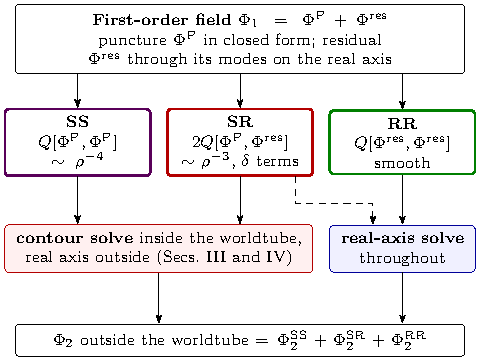
\includegraphics[width=\columnwidth]{fig_flow_overview.pdf}
\caption{Where each piece of the second-order source is solved. The SS and SR pieces, which are singular at the particle, are solved on the complex contour inside the worldtube and on the real axis outside it. The smooth RR piece is solved on the real axis throughout. In the hybrid treatment of SR (Sec.~\ref{sec:hybrid}) only the closed-form part of the source needs the contour; the integrable remainder is formed on the real axis and can be solved there too (dashed arrow). The exterior second-order field is the sum of the linear solves.}
\label{fig:flow}
\end{figure}

Figure~\ref{fig:flow} summarises the strategy.
The first-order field is split into a puncture, known in closed form, and a residual, known through its modes on the real axis.
The SS and SR pieces of the second-order source are put on the contour, by two different methods, and the corresponding mode equations are integrated along it.
The RR piece is smooth and is solved on the real axis, where no shadow can arise.
The exterior second-order field, which is what a flux calculation needs, is the sum of the three.

The paper is organised as follows.
Section~\ref{sec:complex} explains what happens when a real differential equation is integrated in the complex plane: the origin of the shadow, why it is harmless for linear problems and dangerous for quadratic ones, and how the extended delta function, logarithms and kinks in the field each produce shadows of their own.
Section~\ref{sec:ss} presents two ways of putting the SS source on the contour, and relates the second of them to the effective-source method.
Section~\ref{sec:sr} does the same for the SR source, including the hybrid split that avoids the shadow cross term, and assembles the full second-order solution.
Section~\ref{sec:mpu} compares the method with the skeleton-source approach of Musaeus, Pound and Upton, and Sec.~\ref{sec:conclusion} discusses advantages, limitations and future work.
The appendices collect conventions, the consistency conditions on the singular field, a step-by-step account of the angular quadrature at complex radius, and the detailed convergence and cost studies.
Throughout, we write $z$ both for the Cartesian coordinate along the symmetry axis and for the complexified radial coordinate; which is meant is always clear from the context.
The Mathematica implementation used for every result in this paper is available on request.

%=====================================================================
\section{Integrating real equations in the complex plane}\label{sec:complex}

\subsection{The contour and the shadow}\label{sec:shadow}

We decompose every field into axisymmetric spherical-harmonic modes, so that the Laplacian becomes, for each $\ell$, the radial operator $\Lop$ of Appendix~\ref{app:conventions}.
Inside a worldtube of radius $R$ around the particle's radius $r_0$ we replace the radial coordinate $r$ by a complex one,
\begin{equation}
z=y(a)=a+i\eta\Big[1-\frac{(a-r_0)^2}{R^2}\Big]^6,\qquad |a-r_0|\le R,
\label{eq:contour}
\end{equation}
which rises smoothly into the upper half-plane and returns to the real axis at both ends of the worldtube (Fig.~\ref{fig:intro}a).
Outside the worldtube $z$ stays real.
The precise shape of the contour is unimportant; what matters is that it is smooth, that it avoids the particle by a distance comparable to $R$, and that it starts and ends on the real axis.

A point source on the real axis has a natural analytic extension to the complex plane, the extended delta function
\begin{equation}
\dext(z)=\frac{i}{\pi(z-r_0)}.
\label{eq:dext}
\end{equation}
Approached from above, its boundary value on the real axis is the ordinary delta function plus an imaginary principal-value term, $\delta(\Delta r)+\tfrac{i}{\pi}\mathrm{P}(1/\Delta r)$, with $\Delta r=r-r_0$: this is the Sokhotski--Plemelj formula.
The real part is the physical source.
The imaginary part is what we call the shadow of the source.
It is not a small correction; it is of the same order as the physical source, and it has to be understood rather than neglected.

The method rests on one elementary property of linear equations with real coefficients.
Suppose a source is analytic in the region between the contour and the real axis, and that its real part on the axis is the physical source.
Integrate the mode equation along the contour, starting from real data where the contour leaves the axis.
Because the coefficients of the operator are real and analytic there, the solution is also analytic in that region, and taking the real part commutes with the operator.
The real part of the solution's boundary value on the axis therefore solves the real equation with the physical source, and the real parts of the solution and its derivative where the contour rejoins the axis are the physical data from which the exterior solution is continued.
The imaginary part of the solution, the field's shadow, solves the same real equation with the shadow of the source, and in a linear problem it never mixes with the real part.

This simple fact has two consequences that do the work of regularisation.
First, the boundary value from above of an inverse power of $(z-r_0)$ has as its real part the Hadamard finite part of the corresponding inverse power of $\Delta r$~\cite{GelfandShilov}; the finite-part prescription that must be imposed by hand on the real axis is therefore produced automatically by the contour.
Second, the derivative of a kink in a continued field produces a pole of the extended-delta type, as explained in Sec.~\ref{sec:kinks}, so the $\delta$-function content of a source built by differentiating kinked fields appears on the contour without any book-keeping.
Figure~\ref{fig:source} shows the $\ell=2$ SS and SR source modes of the toy model on the real axis and on the contour.
On the axis the SS mode diverges as $\Delta r^{-2}$ and the SR mode has a jump and a $\delta$-function term.
On the contour both are smooth.

\begin{figure*}[t]
\centering
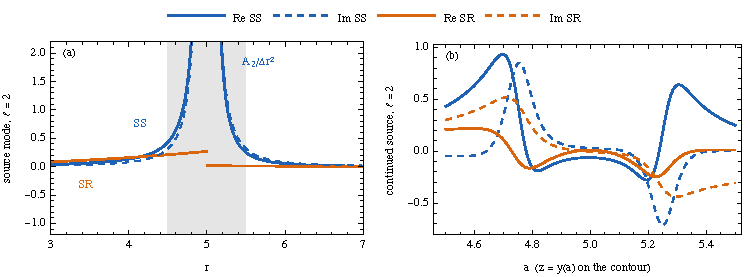
\includegraphics[width=\textwidth]{prl_source.pdf}
\caption{The $\ell=2$ source modes for $q=1$, $r_0=5$ and the regular field $\PhiR=1+z/10$.
(a) On the real axis. SS diverges as $A_2/\Delta r^2$. SR is bounded, with a jump at $r_0$, and also contains a $\delta(\Delta r)$ term with coefficient $c_2=-0.476$ (not shown). The worldtube is shaded.
(b) On the contour $z=y(a)$, with real parts solid and imaginary parts dashed. Both sources are smooth there.}
\label{fig:source}
\end{figure*}

\subsection{Linear versus quadratic problems}\label{sec:quadratic}

For a linear equation the shadow is harmless, and the whole procedure amounts to a convenient way of evaluating a principal-value or finite-part integral: the pole is never approached, no singular quantity is subtracted from another, and ordinary quadrature on the smooth contour suffices.

Quadratic problems are different.
If two continued fields are multiplied on the contour, each being a physical part plus $i$ times a shadow, the real part of the product contains the physical product minus the product of the two shadows.
The shadows are of order one, so this cross term is of order one as well, and it is real.
Taking the real part of the solution at the end of the calculation does not remove it, because the operator has already acted on it.
A second-order source built by multiplying continued first-order fields on the contour would therefore be wrong by an amount set by the shadows of its factors.
Section~\ref{sec:sr} quantifies how wrong, and shows that the error grows with the number of coupled modes.

The way out is to insist that every source on the contour be linear in a single continued quantity.
Each of the three pieces of the second-order source achieves this differently.
The SS piece is a closed-form function of position in three dimensions; it is evaluated at complex radius directly, without ever forming a product of modes.
The SR piece is split into a closed-form part, which is again evaluated at complex radius, and an integrable remainder, which is formed on the real axis from real fields and only then continued onto the contour.
The RR piece is smooth and never goes near the contour.

\subsection{The extended delta function, logarithms and kinks}\label{sec:kinks}

Three closely related objects carry the shadow in this method, and it helps to see how each arises.

\emph{The extended delta function.}
The shadow of $\dext$ is the principal value $\tfrac1\pi\mathrm{P}(1/\Delta r)$.
The first-order mode equation sourced by $\dext$ is solved by the Coulomb mode with its step function at $r_0$ replaced by the continued step
\begin{equation}
H(z)=1+\frac{i}{\pi}\log(z-r_0),
\label{eq:H}
\end{equation}
with the principal branch of the logarithm.
Approached from above, the logarithm of a negative number acquires an imaginary part $i\pi$, so the real part of $H$ is the Heaviside step and its imaginary part, the shadow of the step, is $\tfrac1\pi\ln|\Delta r|$.
The derivative of $H$ is $\dext$, just as the derivative of the step is the delta function.

\emph{Logarithms.}
The shadow of the first-order field is therefore logarithmic at $r_0$, and so is the shadow of every quantity built from it.
The logarithm is also where branch choices enter.
Every logarithm must be placed on the branch whose boundary value from above has the correct real part; Appendix~\ref{app:conventions} gives the one rewriting rule that achieves this, and Appendix~\ref{app:consistency} shows what goes wrong when a computer-algebra system is allowed to choose the branch itself.
In that case the real part of the continued singular mode is not the mode of the three-dimensional singular field but differs from it by a homogeneous solution, which for some $\ell$ is as large as the entire Coulomb field outside the sphere through the particle.

\emph{Kinks.}
The Coulomb mode is continuous at $r_0$ but has a kink there: the mode functions inside and outside are different analytic functions.
A kinked function is continued onto the contour by taking the analytic continuation of the inside piece, adding the difference between the outside and inside pieces multiplied by $H$, and reading the result along the contour.
On the real axis the real part of this blend reproduces the kinked function on both sides of $r_0$.
When the blend is differentiated, the derivative of $H$ produces a term proportional to $\dext$ times the jump in the derivative across $r_0$, and a second derivative produces the derivative of $\dext$ as well.
This is how the $\delta$-function content of the second-order source arises on the contour: the source is built by differentiating kinked fields, and the contour turns each kink into the appropriate pole automatically.
It is also why the blending must be done before the derivatives are taken.
Blending the finished, differentiated source instead discards the $\dext$ terms and gives errors of order one.

Two consistency conditions follow from this discussion, and both are needed for the split into singular and regular fields to mean the same thing on the contour as it does in three dimensions.
The first is that the real part of each continued singular mode on the axis must be the $\ell$-mode of the one three-dimensional puncture used everywhere else, not a convenient particular solution that differs from it by a homogeneous term.
This is the same requirement that real-axis puncture schemes satisfy by construction~\cite{Upton2026}.
The second is that the extended delta function minus the mode operator applied to the continued singular mode must be real on the axis; otherwise the residual field, which is sourced by that difference, acquires a shadow of its own that has nothing to do with the physics.
This condition has no real-axis counterpart.
Appendix~\ref{app:consistency} gives examples of both failures and the homogeneous corrections that cure them.

%=====================================================================
\section{The singular--singular source on the contour}\label{sec:ss}

The SS source is built from the puncture alone, and in the toy model with the exact singular field it is simply the $\partial_z^2$ of $q^2/\rho^2$, up to a factor of a half.
In three dimensions it is a closed-form function of position, singular only on the worldline.
What the contour solve needs, however, is its $\ell$-modes at the contour nodes, and the modes are angular integrals.
On the real axis near $r_0$ those integrals are dominated by a sharp peak at the angle pointing towards the particle, and the modes themselves behave as $A_\ell/\Delta r^2+B_\ell/\Delta r+C_\ell\ln|\Delta r|$.
We compared two ways of obtaining them on the contour, summarised in Fig.~\ref{fig:flowss}.
In the toy model the SS modes are also known in closed form, which is how the two methods are tested, but we deliberately treat the three-dimensional source as the only input, since that is the situation in gravity.

\begin{figure*}[t]
\centering
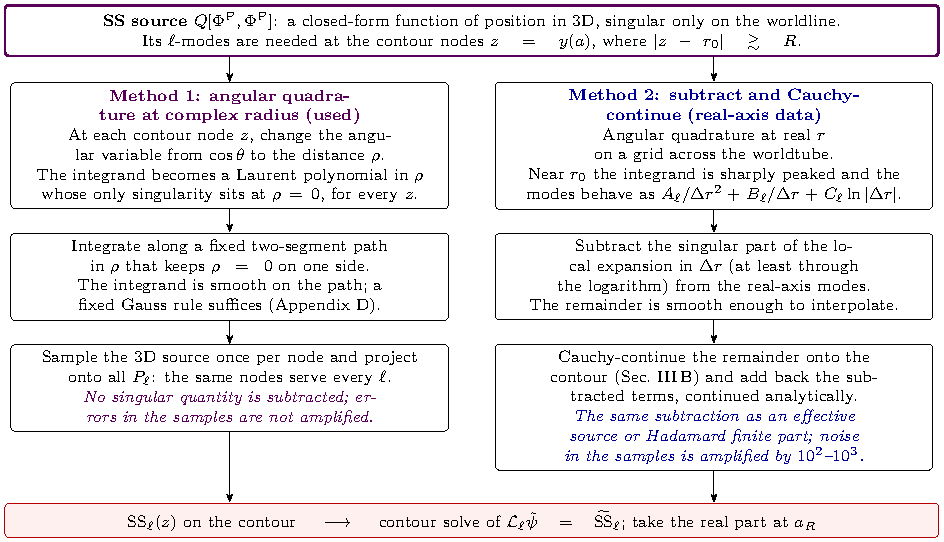
\includegraphics[width=\textwidth]{fig_flow_ss.pdf}
\caption{Two ways of putting the SS source on the contour. Method~1 evaluates the three-dimensional source at complex radius by angular quadrature, with the distance $\rho$ as integration variable; it is the method used in our results. Method~2 starts from real-axis modes, subtracts the singular part of their local expansion, and Cauchy-continues the remainder; it is equivalent in content to an effective-source or Hadamard subtraction.}
\label{fig:flowss}
\end{figure*}

\subsection{Angular quadrature at complex radius}\label{sec:ssquad}

The first method is the one we use.
The three-dimensional SS source is analytic in the radial coordinate at every fixed angle away from the axis; its singularity, where the distance to the particle vanishes, sits at a complex radius whose phase is the angle itself.
We can therefore evaluate the angular integral that defines each mode with the radius set to a contour node, where the integrand is smooth, instead of at a real radius near $r_0$, where it is sharply peaked.

There is one subtlety.
As the contour node moves along the contour, the angle at which the distance to the particle vanishes moves through the complex angle plane, and at the one point where the contour crosses the circle of radius $r_0$ this singular angle lands on the real angular interval over which the mode integral is taken.
A straight integration path in the angle would therefore give a result that jumps as the node passes this point, and the mode would not be an analytic function along the contour.
The cure is to change the integration variable from the cosine of the angle to the distance $\rho$ itself.
The SS source is a Laurent polynomial in $\rho$, the Legendre polynomial becomes a polynomial in $\rho^2$, and the Jacobian is a polynomial too, so the whole integrand becomes a Laurent polynomial in $\rho$ whose only singularity sits at $\rho=0$, for every contour node.
Only the end points of the integration move with the node, and they stay well away from the origin.
A fixed path in $\rho$ that keeps the origin on one side, which we take to be two straight segments through a waypoint on the imaginary axis, then gives the analytic continuation for every node, including the one where the contour crosses the circle.
Which side of the origin the path passes picks out which of the two real-axis branches, inside or outside the particle, is being continued.
For the SS source the two branches differ by a quantity that is imaginary on the axis, so either may be used.
Appendix~\ref{app:quadrature} gives a step-by-step account with a figure, including how the same quadrature handles pieces of the SR source that are kinked at $r_0$.

The result agrees with the closed-form continuation of the SS modes to two parts in $10^{14}$ on the contour, and the exterior field computed from it agrees to the same level.
The integrand is smooth on both segments, so a fixed Gauss rule with 64 to 80 nodes per segment suffices; no adaptive refinement is needed.
Two features of this method matter for cost.
The integration nodes in $\rho$ do not depend on $\ell$, so the three-dimensional source can be sampled once per contour node and projected onto all the Legendre polynomials at once.
And nothing singular is ever subtracted, so errors in the sampled source propagate linearly into the modes and are not amplified.

\subsection{Subtracting the singular part and Cauchy-continuing the rest}\label{sec:sssub}

The second method starts from what a real-axis code already produces: the SS modes on a grid of real radii across the worldtube, computed by angular quadrature at real radius.
Near $r_0$ those modes diverge, so they cannot simply be interpolated onto the contour.
Instead one subtracts the singular part of their local expansion in $\Delta r$, whose coefficients can be computed analytically, continues the smooth remainder onto the contour, and adds back the subtracted terms with $\Delta r$ replaced by $z-r_0$.

The continuation of the remainder is done with a Cauchy integral, and since the same tool is used for the SR source in Sec.~\ref{sec:sr} we describe it here.
Given a real function $s$ on an interval $I$ of the real axis slightly larger than the worldtube, we define its continuation at a complex point $z$ as the convolution of $s$ with the extended delta function,
\begin{equation}
\tilde s(z)=\int_I s(t)\,\dext(z-t)\,dt=\frac{1}{\pi i}\int_I\frac{s(t)}{t-z}\,dt.
\label{eq:cauchy}
\end{equation}
For $z$ in the upper half-plane the integrand is smooth and the integral is an analytic function of $z$.
As $z$ approaches the real axis from above, the Sokhotski--Plemelj formula shows that the real part of $\tilde s$ tends to $s$ itself, while the imaginary part tends to the Hilbert transform of $s$, which is the shadow of $s$.
The continuation therefore has exactly the property the contour solve needs: its real part on the axis is the physical source.
It is linear in the data, it needs $s$ only on the interval $I$, and errors in $s$ propagate into $\tilde s$ without amplification.
Numerically the integral is evaluated by Gauss quadrature after subtracting from $s$ its cubic Taylor polynomial about the real part of $z$, which is integrated against the kernel analytically; this keeps the quadrature accurate when $z$ is close to the axis near the ends of the contour.
The one thing the Cauchy integral cannot do is continue a source that is not locally integrable, or one that contains $\delta$-function terms: a sampled function has no $\delta$ in it, so any $\delta$ content of the true source is simply lost.
This is why the singular part of the SS modes must be subtracted first, and why the SR source cannot be Cauchy-continued whole.
The continuation is also not unique: any function that is analytic between the contour and the axis and whose real part on the worldtube is $s$ would serve equally well, and all such choices differ only in the shadow.
Appendix~\ref{app:cauchy} makes this precise, explains why a Cauchy integral is used rather than a direct analytic continuation, and describes the implementation.

This second method is, in content, the subtraction performed by an effective source or by Hadamard's finite part: the divergent terms are removed analytically and only the remainder is treated numerically.
It works, but the details matter.
Subtracting only the two inverse powers leaves the logarithm in the remainder, which cannot be interpolated accurately, and the error then falls only linearly with the grid spacing.
Subtracting the logarithm as well gives third-order convergence, and subtracting the next two logarithmic terms gives fifth-order convergence, reaching $10^{-14}$ on a grid of spacing $R/100$.
The decisive drawback is noise.
The leading subtracted term grows as $\Delta r^{-2}$, so any error in a sample near $r_0$ is amplified by the same factor before it reaches the remainder.
With a relative noise of $10^{-8}$ on the samples, the level to which the SS source is integrated in current gravitational calculations~\cite{Upton2026}, the continued remainder is wrong by $4\times10^{-5}$: the noise has been amplified by a factor of several hundred to several thousand.
The complex-radius quadrature of Sec.~\ref{sec:ssquad} has no such amplification, which is why we prefer it.
Appendix~\ref{app:ssroutes} collects the convergence and noise results for this route and for a third one, in which a power of $\Delta r$ is factored out of the modes before continuation.

\subsection{What the contour does and does not save}\label{sec:cost}

Since the SS quadrature dominates the cost of current second-order calculations, we measured the cost of computing the exterior SS field in the toy model in several ways, counting evaluations of the three-dimensional source and radial sample points; the tables are in Appendix~\ref{app:ssroutes}.
Three lessons emerge.

The largest saving, by a factor of 200 to 2000 over adaptive angular quadrature performed separately for every mode and every radial point, comes from sampling the source once per radial point and projecting onto all the modes at once.
This saving is available on the real axis as well as on the contour, provided the real-axis integrand is tamed by integrating in a logarithmic distance variable, and it does not require a contour at all.

Per radial point, the cost on the contour is comparable to the cost on the real axis once both use a fixed rule.
The contour's own saving comes from needing fewer radial points: 64 to 80 contour nodes give the exterior field to between $10^{-8}$ and $10^{-12}$, whereas a uniform real grid with the first three singular terms subtracted needs 800 points for $10^{-8}$ and does not reach $10^{-12}$ with 6400.
A real grid graded towards $r_0$, with the same subtraction, matches the contour's count in the absence of noise.

The decisive difference is robustness.
With $10^{-8}$ relative noise on the source samples, the real-axis finite-part integration is between $10^2$ and $3\times10^5$ times less accurate than the contour, because the subtraction amplifies the noise near $r_0$.
The contour samples stay at least a distance $0.3$ from the particle and lose only a factor of 5 to 8.
For a calculation whose source is itself the output of a numerical integration, this robustness, rather than the raw operation count, is the contour's advantage.

%=====================================================================
\section{The singular--regular source on the contour}\label{sec:sr}

The SR source couples the puncture, known in closed form, to the first-order residual field, which is known only through its spherical-harmonic modes on the real axis, up to some maximum coupled mode number $\ell'_{\max}$.
Pointwise it diverges as $\rho^{-3}$, but its angular structure is trace free at leading order, so its $\ell$-modes are bounded: they have a jump at $r_0$ and a $\delta$-function term whose coefficient is proportional to the value of the regular field at the particle.
For $\ell=2$ in the toy model the jump is $-0.254$ and the $\delta$ coefficient is $-0.476$ (Fig.~\ref{fig:source}a).
Figure~\ref{fig:flowsr} summarises the two ways we have tried to put this source on the contour.

\begin{figure*}[t]
\centering
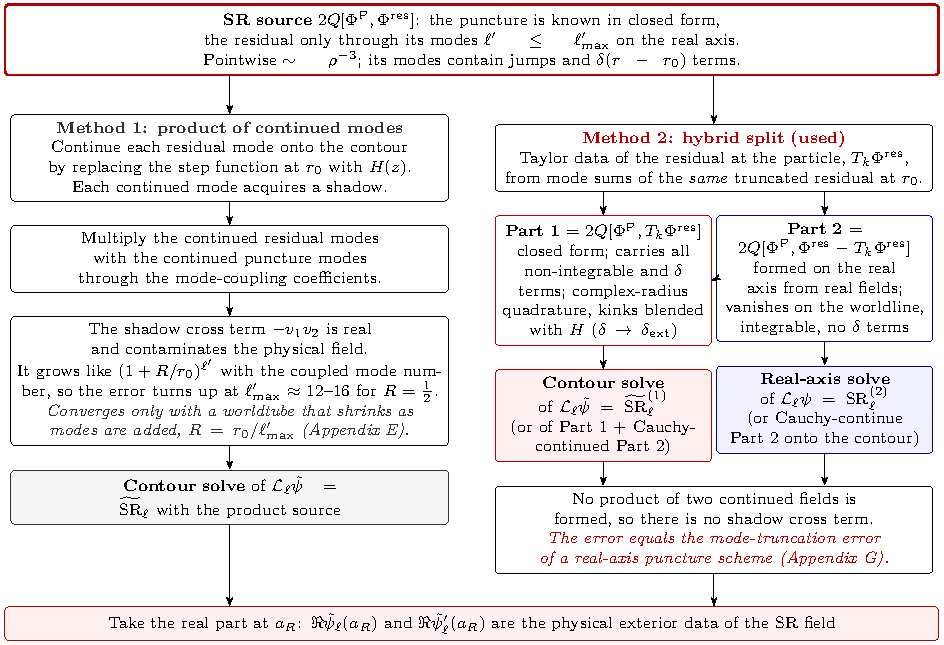
\includegraphics[width=\textwidth]{fig_flow_sr.pdf}
\caption{Two ways of treating the SR source. Method~1 continues the residual modes individually and multiplies them with the continued puncture modes; the product of the two shadows contaminates the physical field, and the contamination grows with the coupled mode number. Method~2, the hybrid split used in our results, separates a closed-form Part~1, which carries every singular and $\delta$-function term and is solved on the contour, from an integrable Part~2, which is formed on the real axis from real fields and solved there (or, equivalently, Cauchy-continued onto the contour and solved with Part~1, dashed arrow); no product of continued fields is ever formed. Both methods end by taking the real part of the contour solution where the contour rejoins the axis.}
\label{fig:flowsr}
\end{figure*}

\subsection{Products of continued modes}\label{sec:product}

The direct approach is to continue each residual mode onto the contour, by writing it as inside and outside pieces blended with the continued step $H$ as in Sec.~\ref{sec:kinks}, and to multiply the continued residual modes with the continued puncture modes through the usual mode-coupling coefficients.
This is exactly the operation that Sec.~\ref{sec:quadratic} warned against, and it fails in an instructive way.

When the puncture is the exact singular field the residual is the smooth injected field, which in the toy model has only $\ell'=0$ and $1$ modes, and the shadow cross term happens to vanish on the axis; the exterior field is then recovered to $3\times10^{-18}$.
With a truncated puncture, which is the realistic case, the residual has modes at every $\ell'$, and each continued mode carries a shadow.
The cross term of the shadows is linear in the truncation error of the puncture, so it shrinks as the puncture is improved, but it grows with the coupled mode number: each coupled mode's contribution grows by a factor of roughly $1+R/r_0$ per unit of $\ell'$, because the inside and outside analytic pieces of a mode of order $\ell'$ grow like that across a worldtube of radius $R$.
For a worldtube of radius one tenth of the orbital radius the total error therefore follows the mode-truncation error up to $\ell'_{\max}\approx12$--$16$ and then turns up (Fig.~\ref{fig:convergence}).
A worldtube that shrinks as modes are added, with radius $r_0/\ell'_{\max}$, keeps the growth factor bounded, and the error then falls monotonically with $\ell'_{\max}$ (Appendix~\ref{app:shadow}).
That is a usable remedy, but an unsatisfying one: it ties the worldtube to the mode truncation, and it still leaves an error that depends on the shadows rather than on the physics.

\subsection{The hybrid split}\label{sec:hybrid}

The method we use removes the cross term altogether.
Let $T_k\Pres$ be the Taylor polynomial of order $k$ of the residual field about the particle.
We split the SR source into two parts,
\begin{equation}
2Q[\PhiP,\Pres]=\underbrace{2Q[\PhiP,T_k\Pres]}_{\rm Part\ 1}+\underbrace{2Q[\PhiP,\Pres-T_k\Pres]}_{\rm Part\ 2},
\label{eq:hybrid}
\end{equation}
where $Q[A,B]$ denotes half of $\partial_z^2(AB)$.

Part~1 is a closed-form function of position, because both the puncture and the Taylor polynomial are, and it can be evaluated on the contour by the same angular quadrature at complex radius as the SS source.
It carries every non-integrable term of SR and every $\delta$-function term, for instance the $\delta$ that comes from the value of the residual at the particle multiplying the second $z$-derivative of the Coulomb field.
Because the mode functions of Part~1 are kinked at $r_0$, the inside and outside branches of the undifferentiated product are blended with $H$ first, and the $z$-derivatives are applied afterwards, so that the $\delta$ terms become $\dext$ poles as described in Sec.~\ref{sec:kinks}.

Part~2 contains the difference between the residual and its Taylor polynomial, which vanishes at the particle like $\rho^{k+1}$ even though the residual itself does not vanish there.
When the operator $Q$ puts two derivatives on the puncture, Part~2 behaves like $\rho^{k-2}$, so for $k\ge0$ it is locally integrable and contains no $\delta$ terms.
In the toy model $k=0$ therefore suffices; a source with more derivatives on the puncture would need a correspondingly higher $k$.
We form Part~2 on the real axis, where both factors are real and no shadow exists.
Being integrable and free of $\delta$ terms, it needs no regularisation at all, and there are two ways to proceed.
The simplest is to treat it like the RR source and solve it on the real axis.
Its modes are integrable but not smooth at $r_0$, where they have logarithmic singularities and jumps, so the real-axis solve must be split at $r_0$ and its quadrature graded towards it, as is standard for such sources; nothing is subtracted, so nothing is amplified.
The alternative, which we used in the tests reported here, is to continue Part~2 onto the contour with the Cauchy integral~\eqref{eq:cauchy} and solve it there together with Part~1, so that the whole of SR is handled by one contour solve with a smooth source.
By the linear-solve property of Sec.~\ref{sec:shadow} the two routes give the same exterior field, and we verified this directly: the contour solve of the continued Part~2 agrees with its real-axis solve to $2\times10^{-16}$ (Appendix~\ref{app:convergence}).
The Cauchy step is cheap, because its kernel does not depend on $\ell$; the continuation is a fixed linear map from the real-axis samples to the contour nodes, built once and applied to every mode.
But it is not necessary, and for a production code the real-axis route is the more economical choice, since it avoids both the continuation and a second source on the contour.
Only Part~1 needs the contour.

One detail makes the split exact rather than approximate.
The Taylor data of the residual at the particle are computed from the same truncated mode sums of the residual at $r_0$ that enter Part~2.
The two parts then add up identically to the truncated SR source, so any error in the local data is absorbed into the ordinary mode-truncation error and the split itself introduces none.
Nowhere in this construction are two continued fields multiplied: Part~1 is linear in a closed-form quantity evaluated at complex radius, and Part~2 is linear in a real function continued by a linear integral.

\begin{figure}[t]
\centering
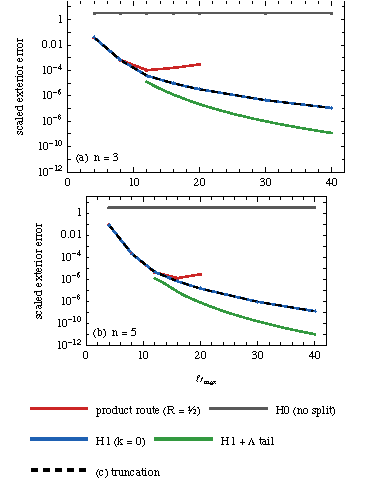
\includegraphics[width=\columnwidth]{prl_convergence.pdf}
\caption{Scaled exterior error against the coupled mode cutoff $\ell'_{\max}$ for the truncated puncture $q/\rho+cq\rho^n$, with (a) $n=3$ and (b) $n=5$, and worldtube radius $R=\tfrac12$.
Red: product of continued modes. Grey: Cauchy continuation of the whole SR source (no split). Blue: hybrid split with $k=0$. Black dashed: mode-truncation error alone. Green: hybrid split with large-$\ell'$ tail fitting.}
\label{fig:convergence}
\end{figure}

Figure~\ref{fig:convergence} compares the two methods, and a third, on punctures truncated in the way a gravitational puncture always is.
We add to the exact singular field a term proportional to an odd power $\rho^n$ of the distance, with a coefficient chosen so that the term is of the natural size $r_0^{-(n+1)}$; the residual is then only $(n-1)$ times differentiable at the particle, and has modes at every $\ell'$.
The product of continued modes follows the mode-truncation error and then turns up, as described above.
Cauchy-continuing the whole SR source, without the split, fails with an error of order one, because the sampled source has lost its $\delta$ terms; the same error, between $0.55$ and $3.3$ for $\ell\le6$, is made by any pointwise real-axis treatment of SR that discards them.
The hybrid split coincides with the mode-truncation error at every $\ell'_{\max}$, and does so for every $k$ from $0$ to $3$.
That error falls as $\ell'^{-(n+2)}_{\max}$, with fitted slopes of $2.93$, $4.87$, $6.83$ and $8.79$ for $n=1$, 3, 5 and 7, and the standard large-$\ell'$ tail fitting~\cite{Upton2026,HeffernanOttewillWardell2012} gains a further factor of 18 to 40 at $\ell'_{\max}=20$.
This is the same algebraic mode-coupling convergence that a real-axis puncture scheme encounters; the contour adds nothing to it (Appendix~\ref{app:convergence}).

\subsection{The regular--regular source and the assembled solution}\label{sec:assembled}

The RR source is built from the residual alone.
It is smooth everywhere, and its modes are computed by coupling real-axis modes in the usual way and solved on the real axis throughout; the contour plays no role.
The exterior second-order field is then the sum of the three linear solves: SS and SR from the contour, RR from the real axis.

With the exact singular field as puncture, and the parameters $q=1$, $r_0=5$, $R=\tfrac12$, $\eta=1$ and $\PhiR=1+z/10$, the assembled exterior modes agree with the exact solution to better than $3\times10^{-18}$ for $\ell\le6$ (Fig.~\ref{fig:solution}).
All radial solves use the boundary conditions that select the solution regular at the origin and decaying at infinity, and the exact solution is adjusted to the same conditions.
As a check that the contour does not introduce any spurious worldline terms, we fitted the SS and SR errors to the modes of a point charge and a point dipole at the particle; the fitted coefficients are below $1.1\times10^{-18}$.
The contour therefore selects the canonical distributional source, with the Hadamard finite part and the full $\delta$-function content and nothing else.

\begin{figure}[t]
\centering
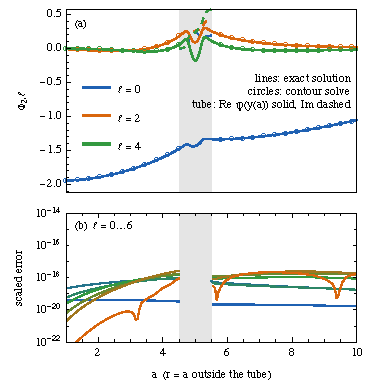
\includegraphics[width=\columnwidth]{prl_solution.pdf}
\caption{(a) Recovered exterior modes $\Phi_{2,\ell}$ (circles) against the exact solution (lines), for an exact puncture, plotted against the contour parameter $a$ ($r=a$ outside the worldtube).
Inside the worldtube the curves show the real (solid) and imaginary (dashed) parts of the contour solution; these are not physical values of $\Phi_2$.
(b) Error scaled by the maximum of each mode, for $\ell=0$--$6$, outside the worldtube.}
\label{fig:solution}
\end{figure}

%=====================================================================
\section{Comparison with the skeleton-source approach}\label{sec:mpu}

Musaeus, Pound and Upton~\cite{MusaeusPoundUpton2026} have recently shown that the second-order field equation can be written with a point-particle source, in which the quadratic Einstein operator acting on the first-order field is replaced by its Hadamard finite part plus a finite term supported on the worldline, which they call $T_Q$ and which is linear in the regular field.
No second-order puncture is needed in their formulation either, so it is natural to ask how the two approaches relate.
They are complementary.
Their work defines the distributional source and shows how to compute its modes on the real axis; ours is a way of integrating the resulting mode equations in which the regularisation happens automatically.
We have made three detailed comparisons.

\emph{The mode-level finite part.}
On their flat-space Teukolsky example, with sources containing inverse powers of $\Delta r$ up to the fourth, we compared their finite-part prescription with an independent Taylor-subtracted finite part and with the contour integral of the Green's function against the source.
The three agree to $4\times10^{-34}$ for $\ell=2$ to $6$, for five choices of worldtube radius and contour height, and their closed form for the $\ell=2$ case is confirmed.
The contour thus reproduces the Hadamard finite part at mode level exactly, as the argument of Sec.~\ref{sec:shadow} says it must.

\emph{The worldline term.}
In the toy model the canonical SR source is a second derivative of an integrable function.
Its four-dimensional finite part is a principal value in which a small ball around the particle is excised, and the difference between the two is a $\delta$ function at the particle with coefficient $-\tfrac{4\pi}{3}q$ times the regular field there; this is the toy model's $T_Q$, and we have verified it to $10^{-21}$.
At the level of modes, the coefficient of the $\delta$ term in each SR mode splits as two thirds from the finite part and one third from $T_Q$.
The reason is that the ball used to define the four-dimensional finite part and the thin shell used to define a mode do not commute for the trace-free $\rho^{-3}$ term of the source.
Their mode-level formula is exact when the mode functions are those of the four-dimensional finite-part distribution.
Applied to pointwise mode functions, however, their mode-level reduction misses the two thirds, and conversely, when source modes are built by coupling kinked mode functions with distributional derivatives, as is done in practice~\cite{Upton2026}, $T_Q$ is already included and adding it again would double count it.
The contour, applied to operators acting on continued integrable functions, yields the canonical source directly, with no separate $T_Q$.

\emph{End-to-end prescriptions.}
Table~\ref{tab:tq} lists the exterior errors of five treatments of the SR source in the toy model with an exact puncture.
The contour and the correct combination of finite-part modes with $T_Q$ both reproduce the exact field; every treatment that omits the $\delta$ content, in whole or in part, fails at order one.

\begin{table}[t]
\caption{Scaled exterior errors ($\ell\le6$) for different treatments of the SR source, with an exact puncture.}
\label{tab:tq}
\begin{ruledtabular}
\begin{tabular}{lc}
prescription & error\\
\hline
contour, canonical source & $<10^{-29}$\\
4D finite-part modes $+\;T_Q$ (their Eq.~24) & $<10^{-19}$\\
4D finite-part modes, without $T_Q$ & $0.18$--$1.1$\\
pointwise modes, their Eq.~105 $+\;T_Q$ & $0.37$--$2.2$\\
pointwise modes, no $\delta$ terms & $0.55$--$3.3$\\
\end{tabular}
\end{ruledtabular}
\end{table}

%=====================================================================
\section{Conclusion}\label{sec:conclusion}

We have shown that continuing each mode equation onto a contour around the particle in the complex radial plane regularises second-order point-particle sources automatically.
The real part of the contour solution on the real axis is the solution of the mode equation with the Hadamard finite part of the source, including every $\delta$-function term, and no second-order puncture is needed.
The difficulty peculiar to second order, that the imaginary shadow of a continued field leaks into the real part of a product, is removed by keeping every contour source linear in a single continued quantity: the closed-form SS source and the closed-form part of SR are evaluated at complex radius by angular quadrature, the integrable remainder of SR is formed on the real axis, where it can be solved directly or continued onto the contour by a Cauchy integral, and the smooth RR source stays on the real axis.
In a scalar model with the distributional structure of the gravitational problem, the method recovers the second-order field to seventeen digits with an exact singular field, and with truncated punctures its error is the mode-truncation error of a real-axis puncture scheme, no more.

The approach has several attractions beyond dispensing with the second-order puncture.
No singular quantity is ever subtracted from another, so numerical noise in the source is not amplified; in our tests the contour was between two and five orders of magnitude more robust to noise in the SS source than real-axis finite-part integration.
The $\delta$-function content of the source, which must be tracked carefully in a real-axis calculation and is easy to lose, is generated by the contour from the kinks in the fields.
And because the angular quadrature nodes at complex radius do not depend on the mode number, the three-dimensional source can be sampled once per radial point and projected onto all modes, a saving that applies equally on the real axis and that may be the most transferable lesson of this work for current gravitational calculations.

The limitations should be stated equally plainly.
The shadow forbids products of continued fields, so a quadratic source can only be handled through a split of the kind described here, and that split relies on the singular part of the source being available in closed form.
The field on the contour itself is not physical; only its real part on the real axis is, so the method as presented delivers the field outside the worldtube, which is what fluxes need, but not the field at the particle.
The toy model is static, scalar and flat, and its exact singular field is a three-term closed form only because the injected regular field is linear; a gravitational puncture is an infinite local series that must be truncated, and the second-order field at a given order of truncation will then converge algebraically rather than exactly.
The gravitational problem also brings azimuthal modes, two-dimensional angular integrals, window functions and logarithmic terms in the puncture, none of which we have tested, although the change of variable to the distance that underlies our angular quadrature appears to carry over to the rotated angular coordinates used for Schwarzschild punctures.
Finally, the per-point cost of the contour quadrature is comparable to a well-designed real-axis quadrature, so the contour is not a short cut to a cheaper SS source; its advantage lies in robustness.

Future work will proceed in two directions.
The first is to apply the method to the Lorenz-gauge and Teukolsky second-order sources in Schwarzschild spacetime, where the complex-radius quadrature of the SS part of the quadratic Ricci tensor would avoid subtracting singular terms from numerically integrated source samples.
The second is to regularise the second-order field itself on the contour.
Because the contour keeps a finite distance from the particle, subtracting a continued second-order puncture from the contour solution there is a difference of two bounded quantities, and the residual can then be continued analytically from the contour back to the particle's radius.
Preliminary tests in the toy model are encouraging: with an exact singular field the continued residual is analytic at the particle and a Taylor series generated from the radial equation converges geometrically to the residual field and its radial derivative there.
This would give access to the regular second-order field at the particle, and hence to the full conservative and dissipative second-order self-force, within the same contour framework that delivers the fluxes.

% TODO: acknowledgments and funding. Re-enable when there is text, otherwise REVTeX prints an empty heading.
%\begin{acknowledgments}
%\end{acknowledgments}

%=====================================================================
\appendix

\section{Conventions and the linear-solve property}\label{app:conventions}
Modes are $\Phi=\sum_\ell\phi_\ell(r)Y_{\ell0}(\theta)$, with $[f]_\ell=\sqrt{\pi(2\ell+1)}\int_{-1}^1 f\,P_\ell(\mu)\,d\mu$ and $\mu=\cos\theta$.
The radial operator is $\Lop=\partial_r^2+\tfrac2r\partial_r-\ell(\ell+1)/r^2$.
The first-order mode source is $\kappa_\ell\,\delta(r-r_0)$, with $\kappa_\ell=-(q/r_0^2)\sqrt{4\pi(2\ell+1)}$.
The Coulomb mode for $\kappa_\ell=1$ is $G_\ell=-r_0^2\,r_<^\ell/[(2\ell+1)r_>^{\ell+1}]$.
With $Q[A,B]=\tfrac12\partial_z^2(AB)$ the source of Eq.~\eqref{eq:model} splits as $Q[\Phi_1,\Phi_1]=\mathrm{SS}+2\,\mathrm{SR}+\mathrm{RR}$, with $\mathrm{SS}=Q[\PhiP,\PhiP]$, $\mathrm{SR}=Q[\PhiP,\Pres]$ and $\mathrm{RR}=Q[\Pres,\Pres]$.
The exact solution is $\Phi_2=\tfrac12\partial_z^2\chi$ with $\nabla^2\chi=\Phi_1^2$; for $\Phi_1=q/\rho+c_0+c_1z$, $\chi=q^2\ln\rho+q(c_0+c_1r_0)\rho+\tfrac12qc_1(z-r_0)\rho+\tfrac16c_0^2r^2+\tfrac15c_0c_1r^2z+\tfrac1{12}c_1^2z^4$.

We use $H(z)$ of Eq.~\eqref{eq:H} with the principal logarithm, and real-axis values are boundary values from above.
Logarithms of the form $\log[c(z-z_*)]$ are rewritten as $\ln|c|+\log(z-z_*)-i\pi[c<0]$.
This is the same function in the upper half-plane, and its principal value on the axis is the value from above.
Without this rewrite, a computer-algebra expression such as $\log(r_0-r)$ at real $r>r_0$ lies on the wrong side of the cut.

\emph{Linear-solve property.}
$\Lop$ has real coefficients that are analytic away from $z=0$.
The solution continued along the contour therefore equals the boundary value from above of the solution in the region between the contour and the real segment.
Taking real parts commutes with $\Lop$, so $\Re\tilde\psi(r+i0)$ solves $\Lop\psi=\Re\tilde s(r+i0)$ with the same real data at $a_L$.
Because $(\Delta r+i0)^{-n}=\mathrm{FP}\,\Delta r^{-n}+i\pi(-1)^n\delta^{(n-1)}(\Delta r)/(n-1)!$, the real part is the Hadamard finite part.

\section{Cauchy continuation of a real-axis function}\label{app:cauchy}

\emph{Definition and boundary values.}
Let $s$ be a real, locally integrable function on an interval $I$ of the real axis that contains the worldtube $[a_L,a_R]$.
Its Cauchy continuation is the convolution of $s$ with the extended delta function, Eq.~\eqref{eq:cauchy}.
Equivalently, one writes $s(r)=\int s(t)\,\delta(r-t)\,dt$ and replaces $\delta$ by $\dext$.
The integral is analytic everywhere off $I$, including the whole upper half-plane.
For $r$ in the interior of $I$ the Sokhotski--Plemelj formula gives the boundary value from above,
\begin{equation}
\tilde s(r+i0)=s(r)-\frac{i}{\pi}\,\mathrm{P}\!\!\int_I\frac{s(t)}{t-r}\,dt,
\label{eq:plemelj}
\end{equation}
so the real part is $s$ itself and the imaginary part, the shadow, is (minus) the finite Hilbert transform of $s$ over $I$.
On the real axis outside $I$ the continuation is purely imaginary, and at large $|z|$ it falls off like $1/z$.
Two special cases recur throughout the paper.
For $s=\delta(t-r_0)$ the continuation is $\dext(z-r_0)$.
For the step $s=\Theta(t-r_0)$ on $I=[a,b]$ it is
\begin{equation}
H_C(z)=\frac{1}{\pi i}\big[\log(b-z)-\log(r_0-z)\big]=H(z)-\frac{i}{\pi}\log(b-z),
\label{eq:HC}
\end{equation}
where we used $\log(z-r_0)=\log(r_0-z)+i\pi$ in the upper half-plane, so that $H(z)$ of Eq.~\eqref{eq:H} equals $\tfrac{i}{\pi}\log(r_0-z)$ there.
The continued step of Sec.~\ref{sec:kinks} and the Cauchy continuation of the step therefore differ by $\tfrac{i}{\pi}\log(b-z)$, a function that is analytic near the worldtube and purely imaginary on the axis for $r<b$.

\emph{What is fixed and what is free.}
The contour solve needs two properties of a continued source $S(z)$: it must be analytic in the closed region between the contour and the segment $[a_L,a_R]$, so that the linear-solve property of Appendix~\ref{app:conventions} applies, and its real part on that segment must be the physical source $s$.
Nothing else is required.
If $S_1$ and $S_2$ both have these properties, their difference $g$ is analytic in the region and has zero real part on the segment.
By the Schwarz reflection principle $g$ then extends analytically across the segment, with $g(\bar z)=-\overline{g(z)}$, and so $g=ih$ with $h$ real-analytic on the segment.
Conversely, adding $ih$ for any such $h$ to an admissible continuation gives another one.
The freedom in the continuation is therefore exactly the freedom to add a pure shadow term.
Its effect on the solution is to add $i\,\delta\psi$, where $\delta\psi$ solves the mode equation with the real source $h$ and is itself real on the axis; the real parts of the solution and its derivative at $a_R$, which are the physical exterior data, are unchanged.
Every admissible continuation gives the same physical field, and ``the'' Cauchy continuation is one representative of this class.
Equation~\eqref{eq:HC} is an example: $H$ and $H_C$ are both admissible continuations of the step and give the same real field.
Other examples are the choice of the interval $I$, since enlarging $I$ changes $\tilde s$ by a Cauchy integral over the added pieces, which is analytic near the worldtube and imaginary on it, and the multiplication of $s$ by a real window that equals one on the worldtube.
If one asks in addition that the continuation be analytic in the whole upper half-plane, have real boundary part equal to $s$ on $I$ and to zero on the rest of the axis, and vanish at infinity, then it is unique and equal to the Cauchy integral: the difference of two such functions would have zero real part on the entire axis and vanish at infinity, so by reflection it would be entire and bounded, hence zero.
The general freedom is thus the freedom to prescribe the real part of the source outside the worldtube and its behaviour at infinity, neither of which enters the physics.

\emph{Why a Cauchy integral rather than an analytic continuation.}
If $s$ were real-analytic on the worldtube, its own analytic continuation $s(z)$ would be admissible, with no shadow at all.
The sources we need to continue are not analytic at $r_0$.
With a truncated puncture, Part~2 of the SR source and the remainder of the SS source in Method~2 are only finitely differentiable there, and even with the exact puncture their modes have kinks.
Such a function has no analytic continuation from the segment.
The Cauchy integral exists for any locally integrable $s$, and it puts the non-smoothness of $s$ into the shadow.
A kink at $r_0$ with a jump $J$ in the first derivative, for instance, produces in $\tilde s$ a term $\tfrac{iJ}{\pi}(z-r_0)\log(z-r_0)$, whose real part on the axis is the kink itself and whose imaginary part is $\tfrac{J}{\pi}\Delta r\ln|\Delta r|$.
More generally a jump in the $(k+1)$th derivative of $s$ produces a shadow term proportional to $\Delta r^{k+1}\ln|\Delta r|$.
The shadow is less smooth than the source, and the solution's shadow inherits this, but by the argument above it does no harm.

\emph{What the Cauchy integral cannot do.}
It requires $s$ to be locally integrable, so the non-integrable terms of a source must be removed before it is applied; this is why Part~1 of the SR split carries them, and why the singular part of the SS modes is subtracted in Method~2.
It also cannot see $\delta$-function terms in a sampled source.
A $\delta$ at $r_0$ continues correctly to $\dext$, but a function known through its samples carries no $\delta$, so the Cauchy continuation of the whole SR source loses the term $c_\ell\dext$ and fails at order one (Sec.~\ref{sec:hybrid}).
Jumps, by contrast, are handled correctly, as Eq.~\eqref{eq:HC} shows.
These two limitations fix the design rule for the split: Part~1 must contain every non-integrable and every $\delta$ term, which is what the condition $k\ge d-2$ guarantees.

\emph{Implementation.}
The real-axis source is represented by Chebyshev interpolants of degree 60 on each side of $r_0$, over the interval $I=[4,6]$ for the worldtube $[4.5,5.5]$.
The interval must extend beyond the worldtube: the Cauchy integral of a function that is cut off at the ends of $I$ has logarithmic singularities there, as $H_C$ has at $z=b$, and if $I$ ended at $a_L$ and $a_R$ these would sit exactly where the contour meets the axis.
For each contour node $z$ the integral is split at $r_0$, the cubic Taylor polynomial of $s$ about $\Re z$ is subtracted and integrated against the kernel analytically, and the remainder is integrated by 80-node Gauss quadrature on each side.
The subtraction matters near the ends of the contour, where $\Im z\to0$ and the kernel becomes nearly singular; subtracting only the value $s(\Re z)$ left an error of $10^{-7}$ that did not converge with the number of nodes.
The continuation is linear in the data, so errors in $s$ propagate into $\tilde s$ without amplification.
Because the kernel does not depend on $\ell$, the continuation is a fixed linear map from the real-axis samples to the contour nodes; it is built once and applied to every mode, so its cost is negligible beside the angular quadrature.
It is also optional: Part~2 is integrable and may be solved on the real axis instead (Sec.~\ref{sec:hybrid}).
As a check, the contour solve of the continued Part~2 agrees with the real-axis solve of Part~2 to $2\times10^{-16}$, less than $10^{-11}$ of the mode-truncation error, for every puncture order and every $\ell'_{\max}$ (Appendix~\ref{app:convergence}).

\section{Consistency of the continued singular mode}\label{app:consistency}
\emph{(i) Real part.}
Any solution $\psi$ of $\Lop\psi=\dext$ satisfies $\Re\psi(r+i0)-G_\ell=\alpha r^\ell+\beta r^{-\ell-1}$, because both sides solve the same real equation with the same $\delta$ source.
The singular structure at $r_0$ does not fix $\alpha$ and $\beta$; the 3D puncture does.

The particular solution returned by \texttt{DSolve} with its integration constants set to zero gives the following ($\ell\le12$ checked):
\begin{itemize}
\item $\ell=0$: an anti-physical Green's function, $(\alpha,\beta)=(r_0,r_0^2)$;
\item $\ell=1$: the Coulomb mode;
\item $\ell\ge2$: a one-sided Green's function that vanishes for $r<r_0$, $\alpha=r_0^{1-\ell}/(2\ell+1)$.
\end{itemize}
Summed in 3D, these offsets give $\Delta=-q/\rho+q\,r\cos\theta/r_0^2-q/r$ for $r<r_0$, and diverge for $r>r_0$.
If such a mode is used with 3D SS and SR, the computed second-order source is $Q[\Phi_1-\Delta,\Phi_1-\Delta]$ instead of $Q[\Phi_1,\Phi_1]$.

\emph{(ii) Imaginary part.}
Replacing the step function by $H$ in the Coulomb mode does not give a solution of $\Lop\psi=\dext$, because $\dext$ is not annihilated by smooth factors that vanish at $r_0$.
For $\ell=0$, $\mathcal L_0[-r_0+(r_0-r_0^2/z)H]=\dext-\tfrac{i}{\pi}z^{-1}$, and the residual field acquires an $O(1)$ shadow, $r/(2\pi)$.
The fix is to add $\tfrac{i}{2\pi}z$.
Equivalently, use the particular solution minus the homogeneous offset found in (i).

\section{Angular quadrature at complex radius, step by step}\label{app:quadrature}
We take the SS source of the model as the example:
\begin{equation}
S(r,\mu)=\tfrac12q^2\,\partial_z^2\rho^{-2}=\tfrac12q^2\big(-2\rho^{-4}+8d^2\rho^{-6}\big),
\end{equation}
where $\rho^2=r^2+r_0^2-2rr_0\mu$ and $d=r\mu-r_0$ is the $z$-component of $\x-\x_0$.
Its modes are
\begin{equation}
\mathrm{SS}_\ell(r)=\sqrt{\pi(2\ell+1)}\int_{-1}^{1}S(r,\mu)\,P_\ell(\mu)\,d\mu.
\label{eq:SSmode}
\end{equation}
The aim is to evaluate this at the contour nodes $r\to z=y(a)$.

\emph{Step 1: where the difficulty comes from.}
At complex $z$ the integrand is singular where $\rho^2=0$, i.e.\ at
\begin{equation}
\mu^*(z)=\frac{z^2+r_0^2}{2zr_0}=\frac12\Big(\frac{z}{r_0}+\frac{r_0}{z}\Big).
\end{equation}
Writing $z=|z|e^{i\varphi}$ gives $\Im\mu^*=\tfrac12\sin\varphi\,(|z|/r_0-r_0/|z|)$.
So $\mu^*$ is real, and lies in $[-1,1]$, exactly when $|z|=r_0$.
Every contour from $a_L<r_0$ to $a_R>r_0$ crosses the circle $|z|=r_0$, at some point $z_c=r_0e^{i\varphi_c}$, where $\mu^*=\cos\varphi_c$ lies on the integration segment.
On either side of $z_c$, $\mu^*$ is on opposite sides of the real $\mu$ axis.
On our contour, $\mu^*$ starts just beyond $\mu=1$ at $a_L$, passes below the segment, through it at $z_c$ and above it, and ends just beyond $\mu=1$ at $a_R$ (Fig.~\ref{fig:quad}a,b).
Integrating along the straight segment $\mu\in[-1,1]$ would therefore jump by $2\pi i$ times a residue as $z$ passes $z_c$, and would not give an analytic function of $z$.
Before $z_c$ the straight segment gives the continuation from $a_L$; after $z_c$ it gives the continuation from $a_R$.
A $\mu$ contour that stays on one branch must keep $\mu^*(z)$ on the same side for every $z$.
For the continuation from $a_L$ it must detour above $\mu^*(z_c)$ at the crossing (violet curve in Fig.~\ref{fig:quad}b), and keep passing above $\mu^*(z)$ afterwards, even where $\mu^*(z)$ has left the axis and the straight segment no longer touches it.
Its shape depends on $z$, so constructing it means following $\mu^*(z)$ along the whole $r$ contour.

\begin{figure*}[t]
\centering
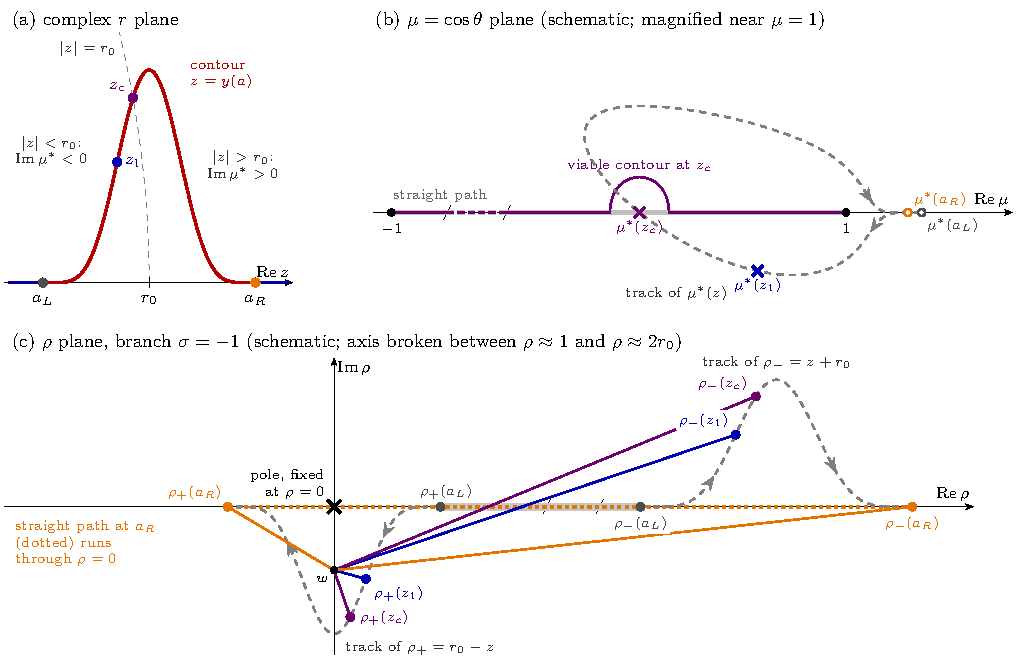
\includegraphics[width=\textwidth]{fig_quadrature.pdf}
\caption{Why the angular integral is done in $\rho$.
Colours mark the points $z_1$, $z_c$ and $a_R$ of the contour in (a), and grey marks $a_L$.
(a)~The contour $z=y(a)$ crosses the circle $|z|=r_0$ at $z_c$.
(b)~The $\mu$ integral runs from $-1$ to $1$; the axis is broken, and the region near $\mu=1$ is magnified.
The dashed curve is the singular angle $\mu^*(z)$ as $z$ runs along the contour.
At real $r$ it lies on the real axis beyond $\mu=1$, outside the integration range (open circles, $z=a_L$ and $a_R$).
Along the contour it passes below the straight path (at $z_1$), through it (at $z_c$) and then above it, so the straight-path integral jumps at $z_c$.
A viable contour must keep $\mu^*(z)$ on the side it started on.
For the branch continued from $a_L$ it must detour above $\mu^*(z_c)$, as shown in violet, and keep passing above $\mu^*(z)$ for every later $z$, even though the straight path no longer touches $\mu^*(z)$ there.
Finding this contour is not straightforward: its shape changes with $z$, and it can only be fixed by following $\mu^*(z)$ along the whole $r$ contour.
(c)~In $\rho$ the pole stays at $\rho=0$; only the endpoints $\rho_-=z+r_0$ and $\rho_+=r_0-z$ move.
The dashed tracks show where they go as $z$ runs from $a_L$ to $a_R$ (arrows), starting from $\rho_\pm(a_L)$ (grey), which are joined by the physical path at $a_L$ (thick grey segment on the real axis).
Each coloured path runs $\rho_-(z)\to w=-i/2\to\rho_+(z)$, the same recipe for every $z$, and never touches the pole.
At $a_R$, $\rho_+=-R$ lies on the real axis on the far side of the pole, and the straight path from $\rho_-$ to $\rho_+$ (orange dotted) runs through it.
The branch $\sigma=+1$ is the mirror image in the upper half-plane.}
\label{fig:quad}
\end{figure*}

\emph{Step 2: change variable from $\mu$ to $\rho$.}
Use the distance from the particle as the integration variable.
From $\rho^2=z^2+r_0^2-2zr_0\mu$:
\begin{gather}
\mu(\rho)=\frac{z^2+r_0^2-\rho^2}{2zr_0},\qquad
d\mu=-\frac{\rho\,d\rho}{zr_0},\nonumber\\
d(\rho)=z\mu-r_0=\frac{z^2-r_0^2-\rho^2}{2r_0}.
\end{gather}
Both $\mu$ and $d$ are polynomials in $\rho^2$, so $P_\ell(\mu(\rho))$ is too, and
\begin{gather}
\mathrm{SS}_\ell(z)=\sqrt{\pi(2\ell+1)}\int_{\rho_-}^{\rho_+}f_\ell(\rho;z)\,d\rho,\nonumber\\
f_\ell=-\frac{\rho}{zr_0}\,S\,P_\ell\big(\mu(\rho)\big).
\label{eq:rhoint}
\end{gather}
The integrand $f_\ell$ is a Laurent polynomial in $\rho$, with powers down to $\rho^{-5}$.
Its only singularity is a pole at $\rho=0$, and this stays \emph{fixed} as $z$ moves along the contour.
Because $S$ and $P_\ell(\mu(\rho))$ depend only on $\rho^2$, $f_\ell$ is odd in $\rho$.

\emph{Step 3: the endpoints.}
$\mu=-1$ maps to $\rho_-=z+r_0$, and $\mu=+1$ maps to $\rho_+=\sigma(z-r_0)$ with $\sigma=\pm1$.
On our contour, $\Re\rho_-\approx2r_0$ and $|\rho_+|=|z-r_0|\ge0.29$, so neither endpoint comes near the pole.
The endpoints move with $z$; the singularity does not.

\emph{Step 4: the path.}
Integrate along two straight segments, $\rho_-\to w\to\rho_+$, with waypoint $w=\sigma i/2$.
For $\sigma=+1$, both $w$ and $\rho_+=z-r_0$ lie in the closed upper half-plane; for $\sigma=-1$, both lie in the closed lower half-plane.
In either case the second segment never meets $\rho=0$, and the first passes at a distance of about $\tfrac12$ from it.
As $z$ moves along the contour, including through $z_c$, the endpoints move continuously and the path never sweeps across $\rho=0$.
By Cauchy's theorem the integral~\eqref{eq:rhoint} is therefore an analytic function of $z$ along the whole contour (Fig.~\ref{fig:quad}c).
Mapped back to the $\mu$ plane, the path is a curve from $-1$ to $1$ that keeps $\mu^*(z)$ on the same side for every $z$, the side being fixed by $\sigma$, like the violet curve in Fig.~\ref{fig:quad}b.
No special treatment is needed at the crossing.
The waypoint matters near the ends of the contour.
A straight path from $\rho_-$ to $\rho_+=r_0-z$ also misses the pole for $z$ in the upper half-plane, but it comes within $0.002$ of it for $a\ge5.4$, and at $a_R$, where $\rho_+=-R$ is real, it runs through it (orange dotted in Fig.~\ref{fig:quad}c).
The path via $w$ can also be deformed, without crossing $\rho=0$, onto a route along the grey tracks in Fig.~\ref{fig:quad}c: back along the track of $\rho_-$ to $\rho_-(a_L)$, along the physical path to $\rho_+(a_L)$, then along the track of $\rho_+$ to $\rho_+(z)$.
That route is the physical path at $a_L$ dragged continuously to $z$, which shows directly that the integral is the continuation from $a_L$.
It would serve equally well as the integration path, but it has three pieces, two of them curved, whose lengths depend on the contour between $a_L$ and $z$; the path via $w$ has two straight pieces and depends only on the current $z$.
Two contours are therefore involved: the $r$ contour, on which the source is needed, and, for each node $z$ on it, a path in $\rho$ for the angular integral.

\emph{Step 5: the two branches.}
Since $f_\ell$ is odd, its antiderivative is even in $\rho$, except for the term $a_{-1}\log\rho$ that comes from the $\rho^{-1}$ term $a_{-1}(z)/\rho$ of $f_\ell$.
The endpoints $\rho_+=\pm(z-r_0)$ therefore give results that differ only through this logarithm, by $\pm i\pi a_{-1}(z)$.
In the $\mu$ plane this is $2\pi i$ times the residue at $\mu^*$: the two branches pass $\mu^*$ on opposite sides.
The same term produces the $\log(z-r_0)$ in the mode function.
\begin{itemize}
\item For real $r<r_0$, the physical path runs along the positive real $\rho$ axis from $r_0+r$ to $r_0-r$, which is the $\sigma=-1$ endpoint. So $\sigma=-1$ continues the inside expression, from $a_L$.
\item For $r>r_0$, the physical endpoint is $r-r_0$, so $\sigma=+1$ continues the outside expression, from $a_R$.
\end{itemize}
For real $z$, $a_{-1}$ is real, so the two branches differ by a quantity that is imaginary on the axis.
For SS, therefore, either branch has the correct real part and can be used.
The $\sigma=+1$ branch agrees with the closed-form continuation of $\mathrm{SS}_\ell$ to $1.8\times10^{-14}$ on the contour.
The $\sigma=-1$ branch differs from it there by 2--30\%, but by a function that is imaginary on the axis, and it gives the exterior field to $2\times10^{-14}$.

\emph{Step 6: pieces with kinks.}
For SR Part 1 the mode functions have kinks at $r_0$, inherited from the Coulomb modes $r_<^L/r_>^{L+1}$.
The inside and outside branches then differ by a real-analytic function, not just by an imaginary term, and neither alone has the correct real part on both sides.
We therefore evaluate both branches of the \emph{undifferentiated} product modes $F_j=[2\PhiP T_k\Pres]_j$, together with their $r$-derivatives at fixed $\mu$, and blend them.
With the jump $J=F_{\rm out}-F_{\rm in}$,
\begin{align}
\tilde F&=F_{\rm in}+JH,\qquad
\tilde F'=F'_{\rm in}+J'H+JH',\nonumber\\
\tilde F''&=F''_{\rm in}+J''H+2J'H'+JH''.
\end{align}
Only then is the $\partial_z^2$ ladder applied in mode space.
The terms with $H'=\dext$ and $H''=\dext'$ carry the $\delta$ content of SR.
This gives the full SR (exact puncture) to $4\times10^{-14}$ and Part 1 to $1.1\times10^{-13}$.
The inside branch alone is wrong by factors of 4 to 1200.
Blending the finished, differentiated source instead loses the $H'$ and $H''$ terms, with errors of 3 to 900.

\emph{Step 7: numerics and cost.}
Each segment uses 80-node Gauss--Legendre quadrature at working precision 30, so each contour node costs 160 evaluations of the 3D source; 64 nodes per segment suffice for $10^{-8}$.
The integrand is a smooth function of $\rho$ on both segments, so no adaptive refinement is needed, and the result is accurate to $10^{-14}$.
The nodes do not depend on $\ell$, so the source can be evaluated once per node and projected onto all modes with the Legendre recurrence.
On the real axis, a fixed rule in $\ln\rho$ does as well per point (56--80 nodes), while adaptive quadrature for each $(\ell,r)$ separately takes 450--3500 evaluations.
The costs are compared in Appendix~\ref{app:ssroutes}.

\emph{Step 8: towards GR.}
In the rotated coordinates $(\alpha,\beta)$ used for Schwarzschild punctures~\cite{Upton2026}, the leading distance at fixed $\beta$ has the form $\rho_0^2=(\Delta r\text{ term})+\chi(\beta)(1-\cos\alpha)$, which is linear in $\cos\alpha$.
Substituting $\rho_0$ for $\alpha$ at fixed $\beta$ should again turn a puncture built from powers of $\rho_0$ and polynomials, including polynomial window functions, into a Laurent polynomial with a fixed pole at $\rho_0=0$.
Terms in $\ln\rho_0$, from higher-order punctures, introduce a branch point instead of a pole. A fixed path with the cut placed away from it should still work.
This extension is untested.

\section{Shadow growth with truncated punctures}\label{app:shadow}
With $\PhiP=q/\rho+cq\rho^n$ used consistently, the real-part mismatch vanishes identically.
The remaining contamination from products of continued modes is linear in $c$.
At fixed $\ell'_{\max}$ it falls by about $0.07$--$0.08$ per unit of $n$, but each coupled mode's contribution grows with $\ell'$.
Near $\ell'=30$ the growth per mode is $1.12$ and $1.19$ for $R=\tfrac12$, and $1.06$ and $1.09$ for $R=\tfrac14$, for the $Q=AB$ and $Q=\nabla A\cdot\nabla B$ toys respectively.
These are close to $1+R/r_0$ times a slowly varying power.

For fixed $R$ the total error therefore has a minimum in $\ell'_{\max}$.
Shrinking the worldtube as modes are added, $R=r_0/\ell'_{\max}$, keeps $(1+R/r_0)^{\ell'_{\max}}$ bounded, and the error then falls monotonically (Fig.~\ref{fig:lprime}).
For $Q=\tfrac12\partial_z^2(AB)$ the minimum lies near $\ell'_{\max}=12$--$16$ (Fig.~\ref{fig:convergence}).
The hybrid split removes the contamination entirely.

\begin{figure*}[t]
\centering
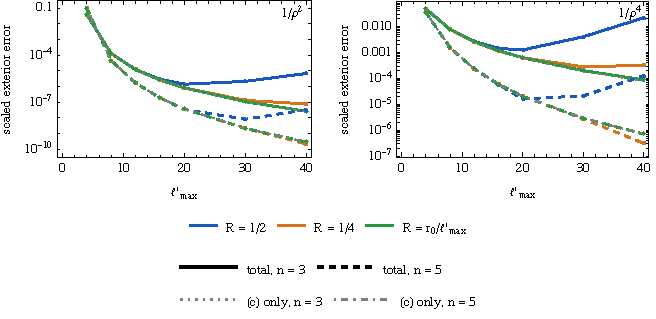
\includegraphics[width=0.75\textwidth]{fig_lprime_optimum.pdf}
\caption{Products of continued modes with a truncated puncture, for $Q=AB$ (left) and $Q=\nabla A\cdot\nabla B$ (right).
Exterior error against $\ell'_{\max}$ for $n=3$ (solid) and $n=5$ (dashed): fixed worldtubes $R=\tfrac12,\tfrac14$, and a shrinking worldtube $R=r_0/\ell'_{\max}$.
Dotted: mode-truncation error.}
\label{fig:lprime}
\end{figure*}

\section{Continuing SS from real-axis data, and the cost of the SS quadrature}\label{app:ssroutes}
\emph{Routes.}
In the toy the SS modes are closed form, so they can be continued directly.
In GR they are available only from numerical angular quadrature.
We compared three ways of putting them on the contour, treating the toy data as if numerical (Fig.~\ref{fig:ssreuse}).
\begin{itemize}
\item \emph{Singular-part subtraction} (Method~2 of Sec.~\ref{sec:ss}). Subtract the singular terms of the local expansion in $\Delta r$, integrate them analytically, and Cauchy-continue the real-axis remainder.
  Subtracting only $A_\ell/\Delta r^2$, or $A_\ell/\Delta r^2+B_\ell/\Delta r$, converges only as $O(h)$ ($9\times10^{-4}$ and $8\times10^{-4}$ at grid spacing $h=0.005$), because the remaining $\ln|\Delta r|$ cannot be interpolated accurately.
  Including $C_\ell\ln|\Delta r|$ gives $O(h^3)$ ($7\times10^{-10}$), and the next two log terms give $O(h^5)$ ($8\times10^{-15}$).
  However, $10^{-8}$ relative noise on the SS samples produces an error of $4\times10^{-5}$: subtracting $A_\ell/\Delta r^2$ amplifies the noise by $3\times10^2$--$4\times10^3$.
\item \emph{Radial factor.} Continue $F_\ell=(r-r_0)^2\mathrm{SS}_\ell$, which is bounded, and divide by $(z-r_0)^2$ on the contour.
  The shadow of $F$ at $r_0$ must be pinned to remove spurious $\delta'$ and $\delta$ terms. Without pinning the error is $5.3$, matching the predicted $-\pi G_0\delta'+\pi G_1\delta$ to $2\times10^{-15}$.
  With exact pinning constants the error is $O(h^3)$. With constants taken from the data, $G_1$ is wrong by $O(h\ln h)$, because of the $\Delta r^2\ln|\Delta r|$ term in $F$, and the method is only first order.
\item \emph{Complex-radius quadrature} (Method~1). Evaluate Eq.~\eqref{eq:SSmode} directly at the contour nodes, as described in Appendix~\ref{app:quadrature}.
  The result agrees with the closed-form continuation to $1.8\times10^{-14}$ on the contour and $2\times10^{-14}$ in the exterior, at a cost similar to real-axis quadrature near $r_0$.
  No singular quantity is subtracted.
\end{itemize}
Summing continued residual modes at complex $r$, $\sum_{\ell'}\tilde\phi^{\rm res}_{\ell'}(z)Y_{\ell'0}(\theta)$, is asymptotically divergent for truncated punctures: terms grow by $1.05$--$1.07$ per $\ell'$ beyond $\ell'\approx30$.
This is why SR Part 2 is formed on the real axis rather than by complex-radius quadrature.

\begin{figure*}[t]
\centering
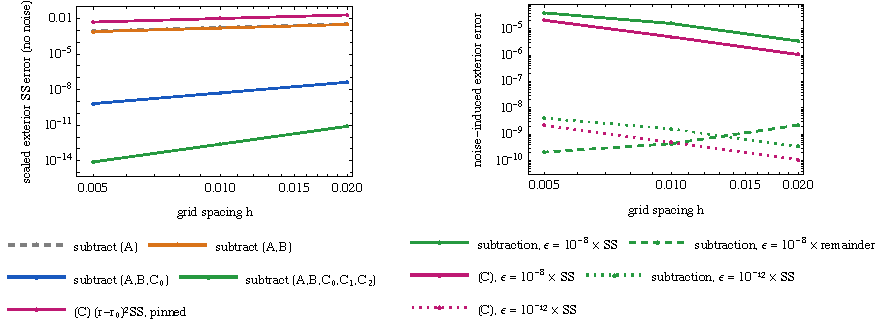
\includegraphics[width=0.85\textwidth]{fig_ss_reuse.pdf}
\caption{Continuing SS from data treated as numerical. Left: error against grid spacing for the subtraction variants and the pinned radial factor. Right: noise propagation.}
\label{fig:ssreuse}
\end{figure*}

\emph{Angular quadrature cost.}
We measured the cost of the SS piece of the exterior field for $\ell\le\ell_{\max}=10$, 20 and 30, on the real axis and on the contour.
Cost is counted as evaluations of the 3D source and as radial sample points.
Errors are maximised over $\ell$ and over exterior points, against the closed form.
Table~\ref{tab:angular} uses the 400-point real grid of spacing $R/200$, as in Ref.~\cite{Upton2026}, and 64 contour nodes.
The first row is the one-dimensional analogue of the adaptive quadrature of Ref.~\cite{Upton2026}.
\begin{itemize}
\item Evaluating the source once per point and projecting it onto all modes is the largest saving, a factor of 200--2000, and it applies on either axis.
\item Per point the costs are similar: 56--80 nodes in $\ln\rho$ on the real axis, against $2\times64$ or $2\times80$ on the contour.
The contour's overall advantage at $10^{-8}$, a factor of 1.2--2.8, comes from its smaller number of radial points.
\item Adaptive quadrature stops short of its own tolerance at high $\ell$.
The contour stalls at $1.6\times10^{-12}$ for $\ell_{\max}=30$, which we do not yet understand.
\end{itemize}

\begin{table}[t]
\caption{Evaluations of the 3D source for the exterior SS field to $10^{-8}$ and $10^{-12}$, $\ell_{\max}=30$.
Adaptive quadrature reaches only $7\times10^{-7}$ and $5\times10^{-10}$ (a, b); the contour stalls at $1.6\times10^{-12}$ (c).}
\label{tab:angular}
\begin{ruledtabular}
\begin{tabular}{lcc}
method & $10^{-8}$ & $10^{-12}$\\
\hline
real axis, adaptive per $(\ell,r)$ & $5.4\times10^6$\,(a) & $5.0\times10^7$\,(b)\\
real axis, shared nodes in $\ln\rho$ & $2.3\times10^4$ & $2.5\times10^4$\\
contour, rule per $\ell$ & $2.3\times10^5$ & (c)\\
contour, shared nodes & $8.2\times10^3$ & (c)\\
\end{tabular}
\end{ruledtabular}
\end{table}

\emph{Radial samples.}
On the real axis the exterior field is the Hadamard finite part of $\int G_\ell\,\mathrm{SS}_\ell\,dr$ over the worldtube.
The terms $A_\ell/\Delta r^2+B_\ell/\Delta r+C_\ell\ln|\Delta r|$ are integrated against $G_\ell$ analytically, and the remainder by quadrature.
This agrees with the contour to $2\times10^{-14}$.
Table~\ref{tab:radial} and Fig.~\ref{fig:radial} give the number of samples needed for $\ell_{\max}=30$; the counts change little with $\ell_{\max}$.
\begin{itemize}
\item Without noise, the real axis can match the contour: a grid graded toward $r_0$ needs 48--120 samples, against 64--80 contour nodes.
A uniform grid needs 100--800, provided the next two logarithmic terms, $\Delta r\ln|\Delta r|$ and $\Delta r^2\ln|\Delta r|$, are also subtracted.
\item With $10^{-8}$ relative noise on the samples, the real-axis result is $10^2$--$3\times10^5$ times less accurate than the contour's.
This noise level matches the accuracy of the numerically integrated SS source in Ref.~\cite{Upton2026}.
Subtracting $A_\ell/\Delta r^2$ amplifies the noise near $r_0$ by the same factor, so the graded grid, which samples closest to $r_0$, suffers most.
Contour samples stay at $|z-r_0|\ge0.3$ and lose only a factor of 5--8.
\end{itemize}

\begin{table}[t]
\caption{Radial source samples needed for the exterior SS field to $10^{-8}$ and $10^{-12}$, and the error when $10^{-8}$ relative noise is added to the samples (at those two configurations).
Uniform grids subtract three terms ($A$, $B$, $C_0$) or five (also $C_1\Delta r\ln|\Delta r|$ and $C_2\Delta r^2\ln|\Delta r|$); with three, 6400 samples give $1\times10^{-11}$.}
\label{tab:radial}
\begin{ruledtabular}
\begin{tabular}{lccc}
method & $10^{-8}$ & $10^{-12}$ & error with noise\\
\hline
contour & 64 & 80 & $8\times10^{-8}$, $5\times10^{-8}$\\
real, graded & 48 & 120 & $4\times10^{-4}$, $1.5\times10^{-2}$\\
real, uniform, 3 terms & 800 & $>6400$ & $9\times10^{-5}$\\
real, uniform, 5 terms & 100 & 800 & $1\times10^{-5}$, $9\times10^{-5}$\\
\end{tabular}
\end{ruledtabular}
\end{table}

% Placed here so that the wide float is encountered early enough to land before the bibliography.
\begin{figure*}[t]
\centering
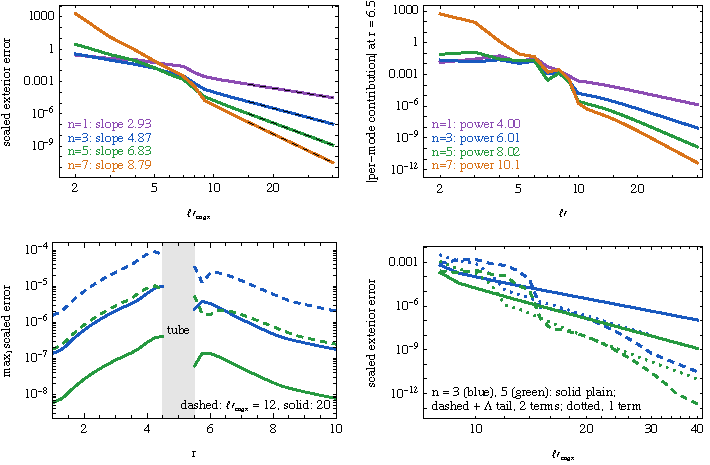
\includegraphics[width=0.85\textwidth]{fig_hybrid_convergence.pdf}
\caption{Hybrid split, $Q=\tfrac12\partial_z^2(AB)$, $k=0$.
Top: error against $\ell'_{\max}$ with fitted slopes, and per-mode contributions against $\ell'$.
Bottom left: error against $r$.
Bottom right: tail acceleration.}
\label{fig:conv}
\end{figure*}

\begin{figure}[t]
\centering
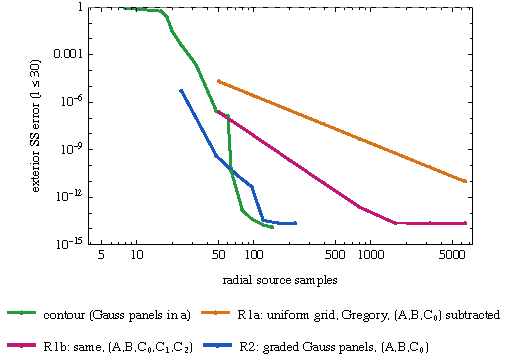
\includegraphics[width=\columnwidth]{fig_radial.pdf}
\caption{Exterior SS error ($\ell_{\max}=30$) against the number of radial source samples, without noise: contour Gauss panels, and real-axis finite-part integration on a uniform grid (with three or five subtracted terms) or on panels graded toward $r_0$.}
\label{fig:radial}
\end{figure}


\section{Convergence of the hybrid split}\label{app:convergence}
With $\PhiP=q/\rho+cq\rho^n$, the residual $\PhiR-cq\rho^n$ is $C^{n-1}$ at $\x_0$.
Its coupled-mode contributions fall as $\ell'^{-(n+3)}$, so the truncation error falls as $\ell'^{-(n+2)}_{\max}$.
The fitted slopes are $2.93$, $4.87$, $6.83$ and $8.79$ for $n=1$, 3, 5 and 7 (Fig.~\ref{fig:conv}).
With the physical boundary conditions used throughout, the error is largest next to the worldtube and decays away from it on both sides.
With Cauchy data at $r=1$ instead, any source error excites the growing solution $r^\ell$, and the error grows towards $r=10$.

Fitting the large-$\ell'$ tail with two terms of the $\Lambda_{\ell,s,n}$ functions of Refs.~\cite{Upton2026,HeffernanOttewillWardell2012} gains a factor of 18--40 at $\ell'_{\max}=20$, and up to 770 at $\ell'_{\max}=30$.
At $\ell'_{\max}=12$ the two-term fit makes the error worse; a one-term fit gains a factor of 2.5--4.3 there.
The hybrid split adds no error of its own: the Cauchy step of the contour solve contributes below $2\times10^{-16}$, less than $10^{-11}$ of the total, and the split error equals the mode-truncation error.

\section{Numerical details}\label{app:numerics}
All computations use working precision 30 and exact rational parameters.
Radial solves use the boundary conditions $\psi'=\ell\psi/r$ at $r=1$ and $\psi'=-(\ell+1)\psi/r$ at $r=10$; for a source on $[1,10]$ these make the free-space Green's function $-r^{\prime2}r_<^\ell/[(2\ell+1)r_>^{\ell+1}]$ exact, and the exact reference is adjusted to the same conditions.
NDSolve is run with PrecisionGoal 20, AccuracyGoal 35 and \texttt{InterpolationOrder -> All}.
Contour sources are evaluated at numerical $y(a)$: symbolic composition expands them into high-degree polynomials and loses all accuracy.
The Cauchy step uses Gauss quadrature after subtracting the cubic Taylor polynomial of $s$ about $\Re z$, which is integrated analytically; the source on the contour is represented piecewise at 40-digit precision.
The implementation is checked by more than 2,500 automated tests.

\begin{thebibliography}{99}
\bibitem{LIGO2016}
B.~P.~Abbott \emph{et al.} (LIGO Scientific and Virgo Collaborations),
Phys.\ Rev.\ Lett.\ \textbf{116}, 061102 (2016).

\bibitem{LISA2017}
P.~Amaro-Seoane \emph{et al.},
arXiv:1702.00786 [astro-ph.IM] (2017).

\bibitem{BarackPound2019}
L.~Barack and A.~Pound,
Rep.\ Prog.\ Phys.\ \textbf{82}, 016904 (2019).

\bibitem{PoundWardell2021}
A.~Pound and B.~Wardell,
in \emph{Handbook of Gravitational Wave Astronomy}, edited by C.~Bambi, S.~Katsanevas, and K.~D.~Kokkotas (Springer, Singapore, 2021).

\bibitem{Pound2012}
A.~Pound,
Phys.\ Rev.\ Lett.\ \textbf{109}, 051101 (2012).

\bibitem{Warburton2021}
N.~Warburton, A.~Pound, B.~Wardell, J.~Miller, and L.~Durkan,
Phys.\ Rev.\ Lett.\ \textbf{127}, 151102 (2021).

\bibitem{Wardell2023}
B.~Wardell, A.~Pound, N.~Warburton, J.~Miller, L.~Durkan, and A.~Le~Tiec,
Phys.\ Rev.\ Lett.\ \textbf{130}, 241402 (2023).

\bibitem{Pound2020}
A.~Pound, B.~Wardell, N.~Warburton, and J.~Miller,
Phys.\ Rev.\ Lett.\ \textbf{124}, 021101 (2020).

\bibitem{MusaeusPoundUpton2026}
J.~Musaeus, A.~Pound, and S.~D.~Upton,
arXiv:2609.10521 [gr-qc] (2026).

\bibitem{MillerWardellPound2016}
J.~Miller, B.~Wardell, and A.~Pound,
Phys.\ Rev.\ D \textbf{94}, 104018 (2016).

\bibitem{BarackGolbourn2007}
L.~Barack and D.~A.~Golbourn,
Phys.\ Rev.\ D \textbf{76}, 044020 (2007).

\bibitem{VegaDetweiler2008}
I.~Vega and S.~Detweiler,
Phys.\ Rev.\ D \textbf{77}, 084008 (2008).

\bibitem{WardellWarburton2015}
B.~Wardell and N.~Warburton,
Phys.\ Rev.\ D \textbf{92}, 084019 (2015).

\bibitem{PoundMiller2014}
A.~Pound and J.~Miller,
Phys.\ Rev.\ D \textbf{89}, 104020 (2014).

\bibitem{Upton2026}
S.~D.~Upton, B.~Wardell, A.~Pound, N.~Warburton, and L.~Barack,
arXiv:2508.00087 [gr-qc] (2026).

\bibitem{DetweilerWhiting2003}
S.~Detweiler and B.~F.~Whiting,
Phys.\ Rev.\ D \textbf{67}, 024025 (2003).

\bibitem{Muskhelishvili1953}
N.~I.~Muskhelishvili,
\emph{Singular Integral Equations} (Noordhoff, Groningen, 1953).

\bibitem{GelfandShilov}
I.~M.~Gel'fand and G.~E.~Shilov,
\emph{Generalized Functions}, Vol.~1 (Academic Press, New York, 1964).

\bibitem{HeffernanOttewillWardell2012}
A.~Heffernan, A.~Ottewill, and B.~Wardell,
Phys.\ Rev.\ D \textbf{86}, 104023 (2012).

\end{thebibliography}

\end{document}
